The \textsc{Nenwin}-scheme is able to simulate a logical NAND-gate.
As a NAND-gate is a Boolean function with only two Boolean input values, there are only 4 different input combinations that need to be handled correctly. Below it is shown how \textsc{Nenwin} can directly simulate a NAND-gate with inputs and output to the \textsc{Nenwin} program itself, and how a NAND-gate can be embedded in a larger circuit within a \textsc{Nenwin}-architecture. 

Let $\mathcal{M}$ denote the set of all possible marbles and $\mathcal{N}$ the set of all possible nodes. 
\begin{lemma}[NAND-gate]
There exists an input placer mapping a vector of two Boolean variables to a set of Marbles $f:\{0, 1\}^2 \rightarrow\mathcal{M}^2$,
a \textsc{Nenwin} architecture of only nodes $A \subseteq \N$, and a function to map the \nenwin output to a Boolean output $g:\mathbb{N}^2 \rightarrow \{\false, \true\}$,\\
such that for two Boolean variables $b_1, b_2 \in \{\false, \true\}$, $g(\vec{y}) = \neg (b_1 \land b_2)$, where $\vec{y}$ is the output harvested from architecture $A$ with input $\{f(b_1), f(b_2)\}$ after all marbles were removes from the network.
\label{lemmma:nand_simple}
\end{lemma}
\begin{proof}

    For all particles we will use \texttt{node\_stiffness} = 0, 
    \texttt{marble\_stiffness} = 1, \texttt{node\_attraction}=0 and \texttt{marble\_attraction}=1.

    Define 
    \begin{equation}
        f(b) = \begin{cases}
            &\texttt{Marble}(pos=[10, 0], vel=\vec{0}, acc=\vec{0}, mass=+10, datum=\textsc{True}) \quad \text{if $b = \textsc{True}$} \\
            &\texttt{Marble}(pos=[10, 0], vel=\vec{0}, acc=\vec{0}, mass=-10, datum=\textsc{False}) \quad \text{if $b = \textsc{False}$}
        \end{cases}
    \end{equation}
    
    Let
    \begin{align}
        A = &[ \nonumber \\
        & \texttt{MarbleEaterNode}(pos=[0, 0], vel=\vec{0}, acc=\vec{0}, mass=+10, radius=5) \nonumber \\
        & \texttt{MarbleEaterNode}(pos=[20, 0], vel=\vec{0}, acc=\vec{0}, mass=-10, radius=5) \nonumber \\
        &]
    \end{align}

    Define 
    \begin{equation}
        g(\vec{y}) = \begin{cases}
                    \false &\text{if } y[0] = 2 \\
                    \true &\text{if } y[0] \in \{0, 1\}
        \end{cases}
    \end{equation}
    
    Note that the Marbles are placed in the middle of the line-segment between the two Nodes, 
    and that positive masses attract positive masses and repel negative masses, and vice versa. 
    Hence each of the two Marbles will be accelerated in a straight line to the Node with the same polarity of mass as itself, 
    and will be eaten by it.
    
    Now if the input is $(\true, \true)$, both Marbles will have a positive mass of 10, and both will be attracted to the left Node (at $pos[0] = 0$ with mass +10). This way both will be absorbed by the first Node, and the output will read $g(\begin{bmatrix}2\\0\end{bmatrix}) = \false$ as expected.
    
    If the input equals $(\true, \false)$, $(\false, \true)$, $(\false, \false)$, then at least one Marble will be attracted and eaten by the right node (at $pos[0] = 20$ with mass -10), and since there are only 2 Marbles, no more than one Marble will be eaten by the left Node, and the output is $g(\begin{bmatrix}1\\1\end{bmatrix})$ or $g(\begin{bmatrix}0\\2\end{bmatrix})$, either of which will evaluate to $\true$ as expected.
\end{proof}
See Fig. \ref{fig:nand_simple} for a visualization of the proof.

\begin{figure}[h]
	\centering
	
\includegraphics[scale=1.5]{figures/nand_simple.pdf}
	\caption{Construction of a NAND-gate in \nenwin as used by the proof of Lemma \ref{lemmma:nand_simple}. The left Node has a positive mass, and the right Node a negative mass. Note that only one dimension (the $x$-axis) is used, and that both Marbles are placed by the input placer on exactly the same position (at $x = 10$).}
	\label{fig:nand_simple}
\end{figure}

The above lemma does not show how a NAND-gate can be implemented as part of a larger circuit. 
To construct a NAND gate that can be used as a submodule, 
it is required that the NAND-gate only attracts particles within a finite region of the real space 
(in case three dimensions are used, this region will be a strict subset of $\mathbb{R}^3$). 
This is needed to ensure that the rest of the circuit can be implemented safely outside this region. 
Furthermore, the NAND gate needs to have interfaces to the other parts of the circuit at the boundary of this region. 

In the following lemma, such interfaces are represented by MarbleEmitterNodes. 
The main advantage of user MarbleEmitterNodes is that it gives more control over how 
the input signal is send into a circuit module (especially in terms of velocity direction), 
in comparison to allowing external Marbles to directly enter the module.

The next lemma will show that is possible to extend the NAND-gate with interfaces to an external circuit. 
It uses a the following encodings for \textsc{True} and \textsc{False}: 
the presence and absence respectively of Marbles with a positive mass (of value $\alpha$). 
Note that the direction and velocity if the Marbles emitted by the output MarbleEmitterNodes can be configured. Furthermore, the NAND-gate requires external 'power' to operate: 
this can be compared to electronic NAND-gates requiring an operating voltage that is separate from the signal. 
This 'power' needs to be the same for each input, and hence does not externally provide information about the input.

\begin{lemma}
    Given positive constants $\alpha \in \mathbb{R}$, a finite cuboid $C \subseteq \mathbb{R}^3$, 
    a finite set of particles in a plane $P \subset C$, and an external Marble $m_{power}$ with a mass of $-\alpha$, 
    \nenwin is able to simulate a NAND-gate using two MarbleEmitterNodes at the boundaries of $C$ as interfaces, 
    such that the particles in $C$ influences no particles beyond $C$ except for creating output Marbles. 
    Here \textsc{True} and \textsc{False} are encoded as presence and absence, respectively, 
    of a Marbles with a mass of $+\alpha$. 
    This NAND-gate creates an output after a finite amount of time, 
    and at this time the NAND-gate returns to a state in which it will produce the same output for the same input.
    \label{lemma:nand_with_iface}
\end{lemma}
\begin{proof}
    The lemma will be proven using a construction. This construction is the concatenation of an AND-gate and a NOT-gate.
    
    Define the following particles in the 'AND' part (also see Fig. \ref{fig:nand_with_iface}). All EmitterNodes and EaterNodes will be initialized with a \texttt{stored\_mass} of 0 and no attraction (which is achieved by setting their \texttt{marble\_attraction} and \texttt{node\_attraction} values to 0\footnote{Alternatively, the state of no attraction could be achieved by giving the Nodes a mass of 0. This distinction is not relevant for the proof.}:
    \begin{itemize}
        \item A signal-emitter: a MarbleEmitterNode in $P$ with a position and radius such that the border of the radius intersects the border of $C$ in one point $p$. This Node functions as the input interface of the NAND-gate, as zero up to two external Marbles serving as input can be consumed by the signal-emitter at point $p$. It has a positive emitting-delay of $\delta \in \mathbb{R}$.
        
        \item A signal-Marble: the Marble that can be emitted by the signal-emitter. It has of mass $\alpha$ with a positive velocity in the direction of the vector from the signal-emitter towards the center of $P$ (this direction will for convenience by called $e_y$ from now, using the axes as in Fig. \ref{lemma:nand_with_iface} we have $up = \begin{bmatrix}x\\ y\\ z\end{bmatrix} = \begin{bmatrix}0\\ 1\\ 0\end{bmatrix}$). The velocity has a magnitude of $v$. It has a Marble-stiffness of 0 and a Marble-attraction of 1.
        
        \item A signal-accumulator: a MarbleEmitterNode in $P$ placed a distance $d_{AND} \in \mathbb{R}^{+}$ from the signal-emitter in the direction $e_y$. $d_{AND}$ is chosen such that the point that is positioned at a positive $d_{NOT}$ in the direction $e_y$ from the signal-accumulator is in $C$. This Node acts as the logic in the AND-part: it emits Marbles with a mass of $2\alpha$, hence it can only emit if the signal-emitter has emitted two Marbles, which only occurs if the signal-emitter has two inputs of value \textsc{True}.
        
        \item A resetter-emitter: a MarbleEmitterNode positioned in $P$, such that it it a distance of $\frac{1}{2}d_{AND} + \psi$ (for a small constant $\psi > 0$) from the center $k$ of the line-segment between the signal-emitter and the signal-accumulator, at a an angle in $(0 \deg, 90 \deg)$ with the line-segment between the signal-accumulator and $k$. It has a radius such that the border of the radius intersects the border of $C$. Note that the signal-accumulator, the signal-emitter and the resetter-emitter are all a distance $\frac{1}{2}d_{AND}$ from $k$. It has an emitting-delay of $2 \delta$.
        
        \item A resetter-Marble that can be emitter by the resetter-emitter, which has a mass of $-\alpha$, a velocity of magnitude $v$ and a velocity-direction towards $k$ from the point where it is emitter. It has a Marble-stiffness of 0 and a Marble-attraction of 1. Since it is directed towards $k$ with the same magnitude of velocity as the signal-Marble, these two Marbles will arrive at $k$ after the same time.
        
        \item An inhibitor-Marble that can be emitted by the signal-accumulator, and that has a velocity with a magnitude $v$ in the direction $e_y$. 
        \item Let $h$ be the point in $P$ that is a distance of $\frac{1}{2}d_{NOT}$ away from the signal-accumulator in the direction $e_y$. It has a Marble-stiffness of 0 and a Marble-attraction of 1.
        
        \item A not-emitter: a MarbleEmitterNode placed in $P$, with a delay of $2\delta + d_{AND} \cdot v$, emitting a Marble (the 'output-Marble') with a mass of $\alpha$ with a velocity with magnitude $v$ in the direction from the not-emitter towards $h$. The not-emitter is positioned such that the line segment between the not-emitter and $h$ has a length of $\frac{1}{2} d_{NOT} + \varepsilon$ (for a small constant $\varepsilon > 0$) and does not intersect any Node nor any line segment between a Node and $k$ or $h$ (see Fig. \ref{lemma:nand_with_iface}). Furthermore, the radius and the position are such that the border of the not-emitter intersects $C$.
        
        \item An output-Marble, as described above, with a Marble-stiffness of 0 and a Marble-attraction of 1.
        
        \item An output-emitter: a MarbleEmitterNode that acts as the output-interface. It is positioned in $P$ such that the line between the output-emitter and the not-emitter intersects $h$, but not any other line segment between a Node and $k$ or $h$, and such that the border of its radius intersects $C$.
        
        \item An accumulator-resetter-1, a MarbleEmitterNode positioned in $P$ such that if the resetter-Marble is repelled by the signal-emitter, its diverted path will lead to the signal-resetter-1. It has a nonnegative delay $\beta$.
        
        \item An accumulator-resetter-Marble, that has a positive velocity $u$ in the direction towards a point $i$ on the line segment between $h$ and the signal-accumulator. It has a mass of $-\alpha$, a Marble-stiffness of 0 and a Marble-attraction of 0. 
        
        \item An accumulator-resetter-2, also a MarbleEmitterNode positioned in $P$, on the ray that originates from the accumulator-resetter-1 and intersects $j$, at a greater distance from the first accumulator than $j$ has. It emits an identical Marble as the accumulator-resetter-Marble, but with a velocity directed towards the signal=accumulator. It has a nonnegative delay $\gamma$.
        
        \item Four garbage-collectors, MarbleEaterNodes all placed in $P$, that only serve to remove unneeded Marbles. One is placed at a distance $d_{NOT}$ in the direction $e_y$ from the signal-accumulator. Another one is placed at a location where the output-Marble will be recoiled towards (when it arrives at $h$ and the inhibitor Marble is at $h$ plus a distance $\varepsilon$ in direction $e_y$). The third one is placed on the ray that originates in the resetter-emitter and intersects $k$, at a greater distance from the resetter-emitter than $k$. The last garbage-collector is placed at a location where the accumulator-resetter-Marble will be recoiled towards from the point $j$, if it arrives at $j$ while the signal-Marble is a distance $\psi$ from $j$ in the direction $e_y$. 
    \end{itemize}
    
    The resetter-emitter and the not-emitter are the part of the gate that requires 'power', i.e. the NAND-gate only functions if these two MarbleEmitterNodes consume Marbles with an equal mass as the Marble they emit respectively, at the same moment as the input is consumed by the signal-emitter. Note that this 'power' can be supplied without disturbing the interior of $C$, as these MarbleEmitterNodes intersect the border of $C$, and the powering Marbles can have a Marble- and Node-attraction of 0.
    
    We now require that, if at some point in time $t_0$ (w.l.o.g. let $t_0 = 0$) the signal-emitter consumes 0, 1 or 2 Marbles with a mass of $\alpha$ (the presence of a Marble encodes the input value \textsc{True}, the absence the input value \textsc{False}), and the resetter-emitter and the not-emitter their required powering Marbles, then the NAND-gate should output a Marble with mass $\alpha$ outside of $C$ at a finite point in time $t_{end} > t_0$, unless two input Marbles are provided. We proceed by a case distinction on the number of input Marbles.
    
    \begin{enumerate}
        \item \textbf{0 input Marbles:} this corresponds to the input $(\textsc{False}, \textsc{False})$. In this case the signal-emitter will not emit any Marble. The resetter-emitter does emit a resetter-marble after a delay of $2\delta$, as it consumes a powering Marble with a mass of $-\alpha$ at the moment $t_0$ at which the empty input is 'given'. However, by construction of the NAND-gate, there is no particle or attraction force on the path of the resetter-Marble except for the garbage-collector, which will consume it. Similarly, the not-emitter will be powered and emit a Marble in the direction of the output-emitter, which will also arrive with its original velocity and direction unaffected at the output-emitter. Hence the \texttt{stored\_mass} of the output-emitter will reach the threshold to emit a Marble with mass $\alpha$ outside of $C$, which encodes the expected output \textsc{True}.
        
        \item \textbf{1 input Marble:} this corresponds to the input $(\textsc{True}, \textsc{False})$, or to the equivalent case $(\textsc{False}, \textsc{True})$. Hence the signal-emitter will emit a signal-Marble with a velocity in the direction of $e_y$. The signal-Marble's velocity will not be affected by the resetter-Marble, since the signal-marble has a Marble-stiffness of 1. There are no other attraction forces or particles along the line segment between the signal-emitter and the signal-accumulator, so the signal-Marble will be consumed by the signal-accumulator. This causes the signal-accumulator to obtain a \texttt{stored\_mass} of $\alpha$, which is not sufficient for it to emit a Marble.
        
        The resetter-emitter will also emit a resetter-Marble, which will arrive at the point $k$ when the signal-Marble is a distance $\psi$ in the direction $e_y$ from $k$ (this is, because both Marbles are emitted at the same time in a straight line to $k$ with the same velocity $k$, only the resetter-emitter needs to travel an additional distance $\psi$). If the the attraction threshold distance of the signal-Marble and the value of $\psi$ have been chosen correctly, then the resetter-Marble will be recoiled by the signal-Marble in a direction different than its original direction (as the signal-Marble is positioned in the direction of $e_y$ from the resetter-Marble, and the repelling force accelerated the resetter-Marble in the direction of the line from the signal-Marble to the resetter-Marble). So by construction the resetter-Marble will be redirected towards the accumulator-resetter-1 (the green arrow in Fig. \ref{fig:nand_with_iface}, which in turn will emit a Marble towards the accumulator-resetter-2, which in turn will emit a Marble towards the signal-accumulator. Since this Marble has an opposite mass as the signal-Marble that the signal-accumulator consumed, its \texttt{stored\_mass} will be reset to 0. It is possible that the negatively-massed Marble will be consumed before the signal-Marble instead, but clearly this leads to the same result \footnote{Alternatively, $\gamma$ (the delay of the accumulator-resetter-2) can be adjusted to ensure the signal-Marble will be consumed by the signal-accumulator first. This does not affect the resulting state of the particles of the NAND-gate.}. 
        
        The rest of the NAND-gate behaves identical as the case of \textit{0 input Marbles}, which leads to the correct output at the output-emitter.
        
        \item \textbf{2 input Marbles:} this corresponds to the input $(\textsc{True}, \textsc{True})$. In this case two signal-Marbles will be emitted, at $t = t_0 + \delta$ and at $t = t_0 + 2\delta$. As in the case of \textit{1 input Marble}, the first signal-Marble will be consumed by the signal-accumulator, and the resetter-Marble will be consumed by the accumulator-resetter-1. Now there exists a value for $\beta$ (the delay of the accumulator-resetter-1) such that there exists a small constant $\omega > 0$ such that the second signal-Marble is a distance $\omega$ in the direction $e_y$ from $j$ when the accumulator-resetter-Marble arrives at $j$. Similarly to the redirection of the resetter-Marble, this causes the accumulator-resetter-Marble to be redirected, which by construction sends the accumulator-resetter-Marble towards a garbage-collector (the yellow line in Fig. \ref{fig:nand_with_iface}).
        
        Hence the signal-accumulator will consume two Marbles each with a mass of $\alpha$ at $t = t_1 = t_0 + 2\delta +  d_{AND}\cdot v$ (where $d_{AND}\cdot v$ is the time needed for the second signal-Marble to travel from the signal-emitter to the signal-accumulator), but the accumulator-resetter-emitter-2 will not emit a Marble with negative mass, hence at $t_1$ the signal-accumulator will emit an inhibitor-Marble. This is also the time at which the not-emitter emits an output-Marble. 
        
        Similar to the first signal-Marble, the resetter-Marble and the point $k$, the output-Marble will arrive at the point $h$ when the inhibitor-Marble is a distance $\varepsilon$ in the direction $e_y$ from $h$. The inhibitor-Marble has a Marble-stiffness of 1, but the output-Marble has a Marble-stiffness of 0 and hence there exists a threshold distance for the inhibitor-Marble and a value for $\varepsilon$ such that the output-Marble will be shortly accelerated in the direction of the inhibitor-Marble. Then by construction, the output-Marble will be redirected to an garbage-collector (the purple line in Fig. \ref{fig:nand_with_iface} instead of the output-emitter. Also by construction, the inhibitor-Marble travels in a straight line from the signal-accumulator to a garbage-collector. Hence both particles will be consumed by garbage-collectors. Note that also the signal-accumulator now has a \texttt{stored\_mass} of 0, as the previously stored mass of $2\alpha$ has been depleted when emitting the inhibitor-Marble. 
        
        It can be concluded that, after the amount of time passed in which the NAND-gate produced output in the \textit{0 input Marbles} and \textit{1 input Marble} cases (which is the same time-span for both cases), no output will be produced, as required by the definition of a NAND-gate.
    \end{enumerate}
    Note that in all three cases, the NAND-gate eventually returned to the same state as before the input was given, except for the amount of Marbles eaten by the garbage-collectors. But the latter does not affect the behaviour of the NAND-gate, hence it will respond with the same outputs again given any of the three input cases above.
\end{proof}
\clearpage
\begin{figure}[h]
    \centering
    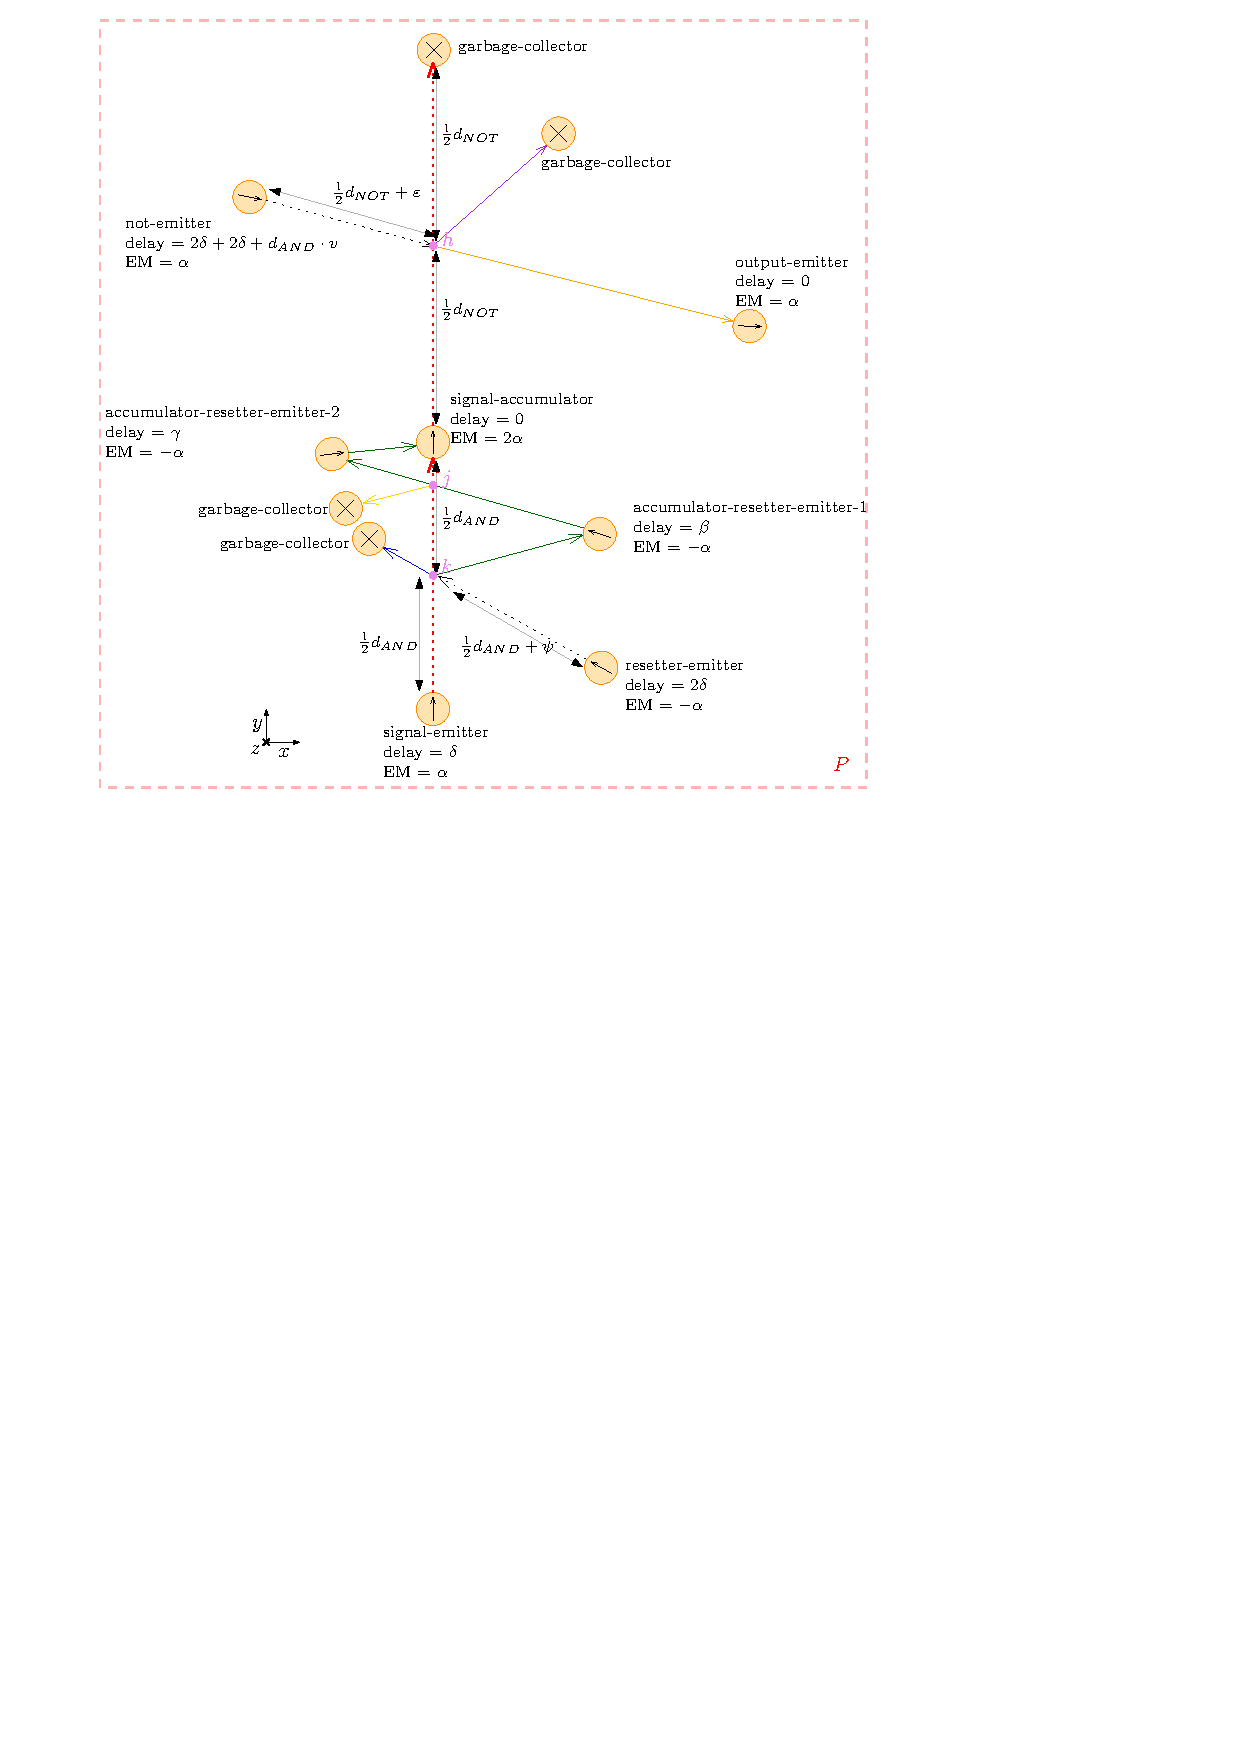
\includegraphics{figures/nand_with_interfaces_v6.pdf}
    \caption{Construction of a NAND-gate in \nenwin as used by the proof of Lemma \ref{lemma:nand_with_iface}. The axes of spatial coordinates $x$ and $y$ are parallel to the place $P$. For each MarbleEmitterNode, the emit-delay and the mass of the emitted marble (EM, 'Emitted Mass', for short) have been denoted. MarbleEmitterNodes are marked with an arrow that indicates the direction of the velocity of the Marble they can emit, and the MarbleEaterNodes (that is not also an EmitterNode) has been marked with a cross. Note that the distances between particles and the radii of the Nodes are not to scale.}
    \label{fig:nand_with_iface}
\end{figure}
\clearpage